\documentclass{beamer}
\usepackage{hyperref}
\usepackage{animate}
\usepackage{amsmath}
\usepackage[T1]{fontenc}
\usefonttheme[onlymath]{serif}
\usepackage[spanish,provide=*]{babel}
% Cargar apacite después de babel para citas autor-año correctas
\usepackage[notocbib]{apacite}

% other packages
\usepackage{latexsym,amsmath,xcolor,multicol,booktabs,calligra, tcolorbox}
\usepackage{graphicx,listings,stackengine}
% Manejo robusto de nombres de archivo con espacios y rutas de imágenes
\usepackage{grffile}
%\graphicspath{{pic/}}

\renewcommand{\APACrefbtitle}[2]{#1}       % Muestra solo el título 
\renewcommand{\APACrefYearMonthDay}[3]{#1} % Muestra solo el año (omite mes/día)

\author{Dylan Jara}
\title{Analisis de la fisica para la creacion de una PINN para prediccion de lahares y
de mapas de peligro volcanico}
\subtitle{}
\institute{
    Universidad de Santiago de Chile
}
\date{\today}
\usepackage{../Ritsumeikan}

% defs
\def\cmd#1{\texttt{\color{red}\footnotesize $\backslash$#1}}
\def\env#1{\texttt{\color{blue}\footnotesize #1}}
\definecolor{deepblue}{rgb}{0,0,0.5}
\definecolor{ccnuMainColor}{RGB}{57,64,73}
\definecolor{deepgreen}{rgb}{0,0.5,0}
\definecolor{halfgray}{gray}{0.55}

\lstset{
    basicstyle=\ttfamily\small,
    keywordstyle=\bfseries\color{deepblue},
    emphstyle=\ttfamily\color{ccnuMainColor},    % Custom highlighting style
    stringstyle=\color{deepgreen},
    numbers=left,
    numberstyle=\small\color{halfgray},
    rulesepcolor=\color{red!20!green!20!blue!20},
    frame=shadowbox,
}

\renewcommand{\APACrefbtitle}[2]{#1} % Muestra solo el título
\renewcommand{\APACrefYearMonthDay}[3]{#1} % Muestra solo el año
\renewcommand{\APACrefnote}[1]{} % Elimina las notas

\begin{document}

\begin{frame}
    \titlepage
    \vspace*{-0.6cm}
    \begin{figure}
        \begin{center}
                % Ajuste de tamaño más visible y uso de \graphicspath
                
\includegraphics[keepaspectratio, width=0.25\textwidth]{./Pics/Usach S1.png}

        \end{center}
    \end{figure}
\end{frame}

% Restaurar la tabla de contenidos y corregir el problema de 'Referencias32'
\begin{frame}
    \tableofcontents[sectionstyle=show, subsectionstyle=show/shaded/hide]
\end{frame}

%//////////////////////////////////////////////////////%
\section{Introducción}
\subsection{Lahares}
\begin{frame}{Qué son los lahares?}
    \begin{itemize}
        \item<1-> Volcanic debris flows that originate at potentially active volcanoes are called lahars \cite{Vallance2024}.
        \item<2-> Lahars are mixtures of water, volcanic ash, tephra, rock fragments, and chunks of ice that can flow like wet concrete. 
        \item<3-> The term comes from the Indonesian word for these destructive mudflows that cause both property damage and loss of life.
    \end{itemize}
\end{frame}

\begin{frame}
    \begin{figure}
        \centering
        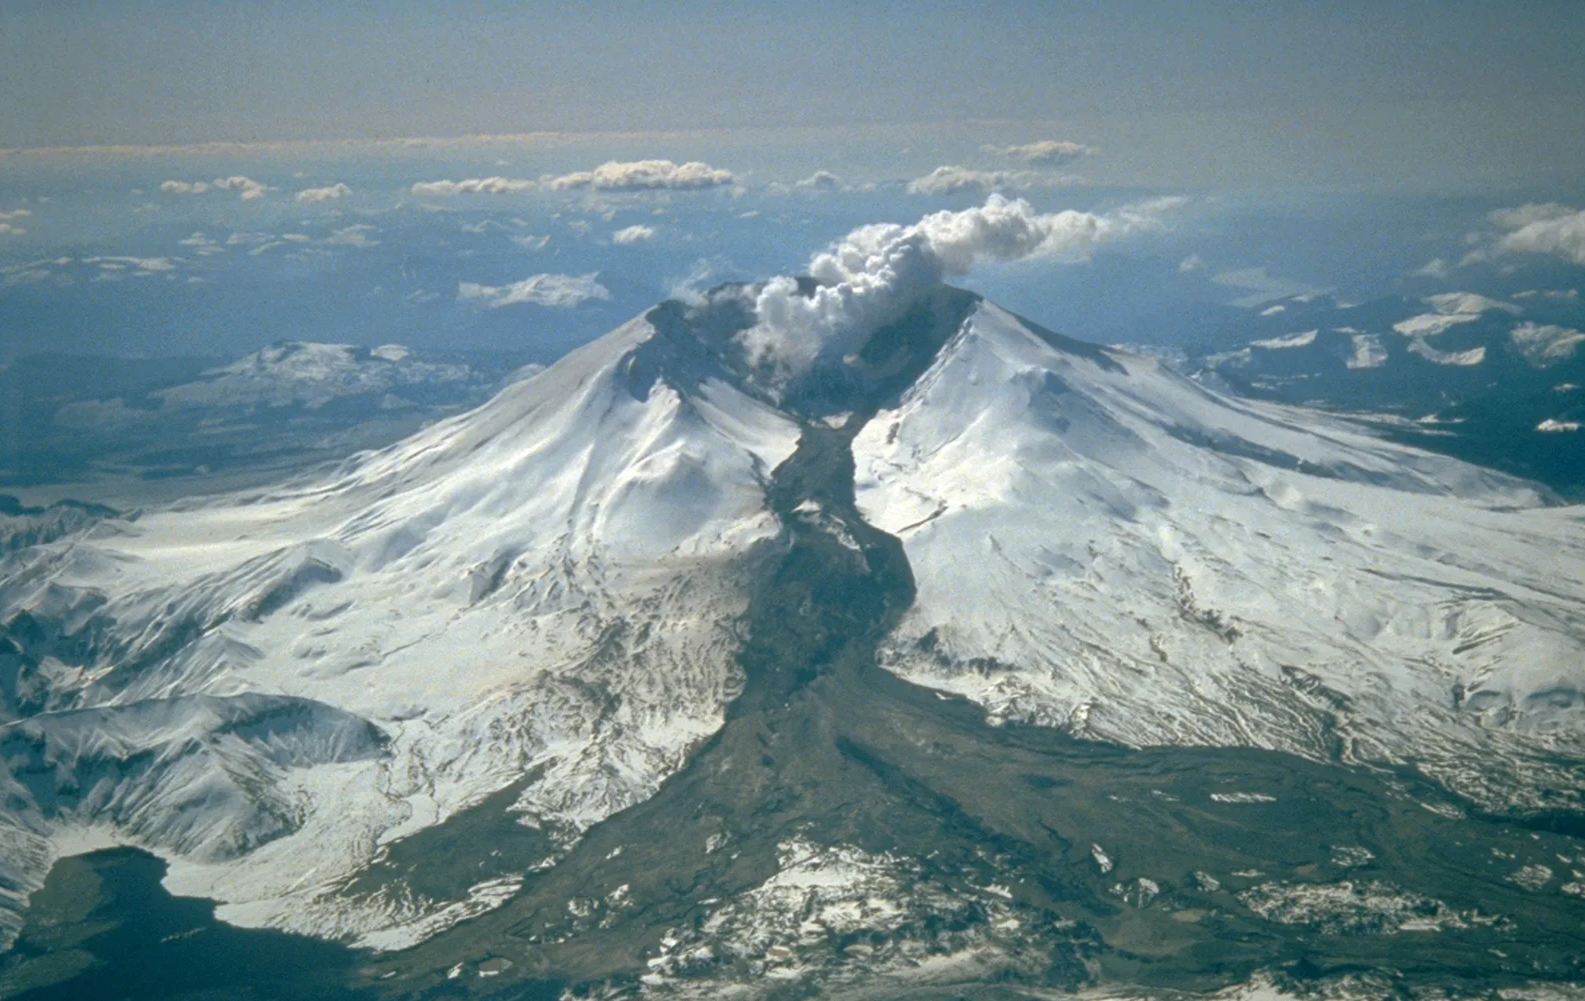
\includegraphics[width=10cm,height=6cm]{.//Pics//lahar.png}
        \caption{Lahar (dark deposit on snow) on Mount Saint Helens after the March 19, 1982, eruption.}
    \end{figure}
\end{frame}


%/////////////////////////////////////////////%
\section{Estado del Arte}
\begin{frame}{Metodos numericos actuales para prediccion}
\begin{itemize}
    \item LAHARZ es un modelo computacional que utiliza descripciones estadísticas de áreas inundadas por eventos pasados de flujo masivo 
para pronosticar áreas que probablemente serán inundadas por eventos hipotéticos futuros. \cite{schilling2008using}
    \item D-Claw es una biblioteca de software para la simulación de flujos granulares densos sobre topografía espacialmente variable. \cite{george2025d}
    \item LaharFlow es un software de dinámica de lahares, diseñado en la Universidad de Bristol, que
modela el flujo de lahar como una mezcla de agua y granos sólidos, basado en tres principios
de conservación. Estos son conservación de la masa, momentum y transporte de material sólido \cite{woodhouseshallow}
\end{itemize}

\end{frame}


%/////////////////////////////////////////////%
\section{Modelos, ANN y PINNs}
\begin{frame}{Ecuaciones Shallow-water}
\begin{itemize}
    \item Son un sistema de PDEs hiperbolicas que describen el flujo de fluidos en oceanos, rios, etc.
    \item Se caracterizan ya que su dimension vertical es mucho menor que la horizontal, lo que permite simplificar las ecuaciones de Navier-Stokes.
    \item Se utilizan para modelar fenómenos como tsunamis, mareas, debris flows, etc.
    \item Provienen de la derivacion de Navier-Stokes, que a su vez provienen de las leyes de conservacion de masa, momentum.
\end{itemize}
\end{frame}

\begin{frame}{Que son las PINNs?}
\begin{itemize}
    \item Physics-informed neural networks are neural networks that are trained to solve supervised learning tasks while respecting
    any given laws of physics described by general nonlinear partial differential equations. \cite{RAISSI2019686}
    \item Such neural networks are constrained to respect any symmetries, invariances, or conservation principles originating from
the physical laws that govern the observed data, as modeled by general time-dependent and nonlinear partial differential
equations.
\end{itemize}
\end{frame}



\begin{frame}
    \begin{figure}
    \centering
    % {12} es la velocidad (cuadros por segundo)
    % [0-49] asumiendo que tu PDF tiene 50 páginas (índice empieza en 0)
    \animategraphics[autoplay,loop,width=\linewidth]{20}{./Pics/pinnpdf}{0}{49}
    \caption{Simulación PINN: Evolución del flujo.}
\end{figure}
\end{frame}

\begin{frame}{PDEs y Residuos en la PINN}
\begin{itemize}
    \item $\mathcal{L} = \mathcal{L}_{data} + \lambda \mathcal{L}_{physics}$, donde $\mathcal{L}_{data}$ mide el error en los datos y $\mathcal{L}_{physics}$ mide el incumplimiento de las PDEs.
\end{itemize}
\end{frame}

\section{Variables y parámetros}
\begin{frame}{Variables y parámetros}
\begin{itemize}
    \item $h(x, y, t)$: espesor de la mezcla $(m)$,
    \item $u(x, y, t), v(x, y, t)$: velocidades promediadas en profundidad $(m/s)$,
    \item $C(x, y, t)$: concentración volumétrica de sólidos $(\text{adimensional}, 0 \leq C \leq 1)$,
    \item $z_b(x, y, t)$: elevación del lecho $(m)$.
\end{itemize}
\end{frame}

\section{Physics-Informed Neural Networks (PINNs)}
\subsection{Sistema acoplado de PDEs}
\begin{frame}{Conservacion de Masa}
Conservacion de masa con fuente de masa: 
    \begin{align}
    {\partial h \over \partial t} + \nabla \cdot (h \vec{u}) = S_h(x,y,t), && u=(u,v)
    \end{align}
\end{frame}

\begin{frame}{Conservacion de Momentum}
Conservacion de momentum 2D con friccion basal modulada:
    \begin{align}
    {{\partial u} \over{\partial t}}+u{{\partial u} \over{\partial x}}+v{{\partial u} \over{\partial y}}+g{{\partial H} \over{\partial x}}+{{\tau_{bx}} \over{\rho_mh}} = 0 \\
    {{\partial v} \over{\partial t}}+u{{\partial v} \over{\partial x}}+v{{\partial v} \over{\partial y}}+g{{\partial H} \over{\partial y}}+{{\tau_{by}} \over{\rho_mh}} = 0
    \end{align}
    Donde la tension basal es parametrizada como 
    \begin{align}
    \tau_{b} = \tau_{b}\frac{u}{\|u\|+\epsilon},&&\tau_{b}=\mu_{eff}(C,p)\rho_mgh \cos\theta
    \end{align}
\end{frame}

\begin{frame}{Conservacion de Momentum}
    La pendiente se aproxima por:
    \begin{align}
        \cos\theta\approx \frac{1}{\sqrt{1+\|\nabla z_b\|^2}}
    \end{align}
    Un modelo reducido pero físicamente interpretable para fricción efectiva:
    \begin{align}
        \mu_{eff}(C,p) = \mu_0(1+\alpha_C(C-C_0))\exp(-\alpha \frac{p}{\rho_mgh+p_{ref}})
    \end{align}
    donde C0 es una concentración de referencia y pref estabiliza la razón. Este término representa: (i) mayor fricción con mayor carga sólida, y 
    (ii) menor fricción efectiva cuando el exceso de presión de poros es alto (disminuye el esfuerzo efectivo).

\end{frame}

\begin{frame}{Ecuacion de transporte de solidos (Adveccion-difusion)}
    Ecuación advección–difusión con término de relajación hacia un equilibrio
    \begin{align}
    {\partial C \over \partial t} + u\cdot \nabla C = \nabla \cdot (k_C\nabla C) + \frac{C_{eq}(x,y)-C}{\tau_C}
    \end{align}
    En prototipo sintético se puede fijar $\tau C \rightarrow \infty$ (sin relajación) o definir $C_{eq}$ como mayor en cauces y menor en planicies.
\end{frame}


\begin{frame}{Evolucion de presion de poros}
    \begin{figure}
    \centering
    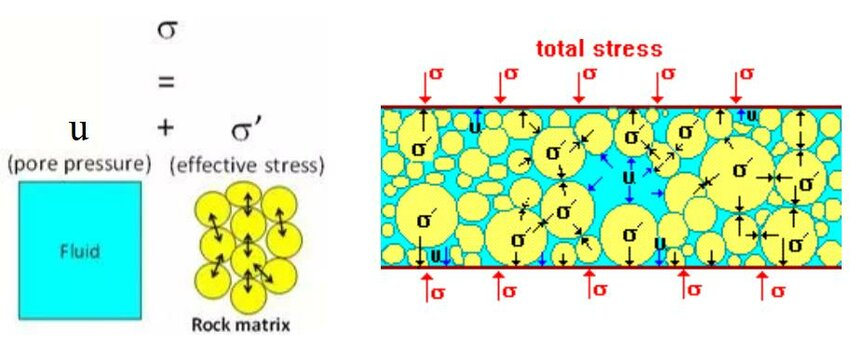
\includegraphics[width=10cm,height=6cm,keepaspectratio]{.//Pics//porepressure.png}
    \caption{Diagram illustrating the effective stress principle in a saturated cohesionless soil \cite{phdthesis}}
    \end{figure}
\end{frame}
\begin{frame}{Evolucion de presion de poros}
    Se usa una ecuación de advección con relajación:
    \begin{align}
    {\partial p \over \partial t} + u\cdot \nabla p = \frac{p_{eq}(h,C,\|u\|)-p}{\tau_p}
    \end{align}
    Un ejemplo simple para equilibrio de presión:
    \begin{align}
        p_{eq}=\chi_p\rho_m gh\phi(C)\frac{\|u\|}{\|u\|+u_*}, && \phi(C)=\frac{C}{C+C_*}
    \end{align}
    que aumenta con espesor y con concentración, y satura con velocidad. Esto captura cualitativamente el aumento de presión por mezcla densa y cizalle.
 
\end{frame}


\begin{frame}{Ecuacion de Exner}
    \begin{figure}
    \centering
    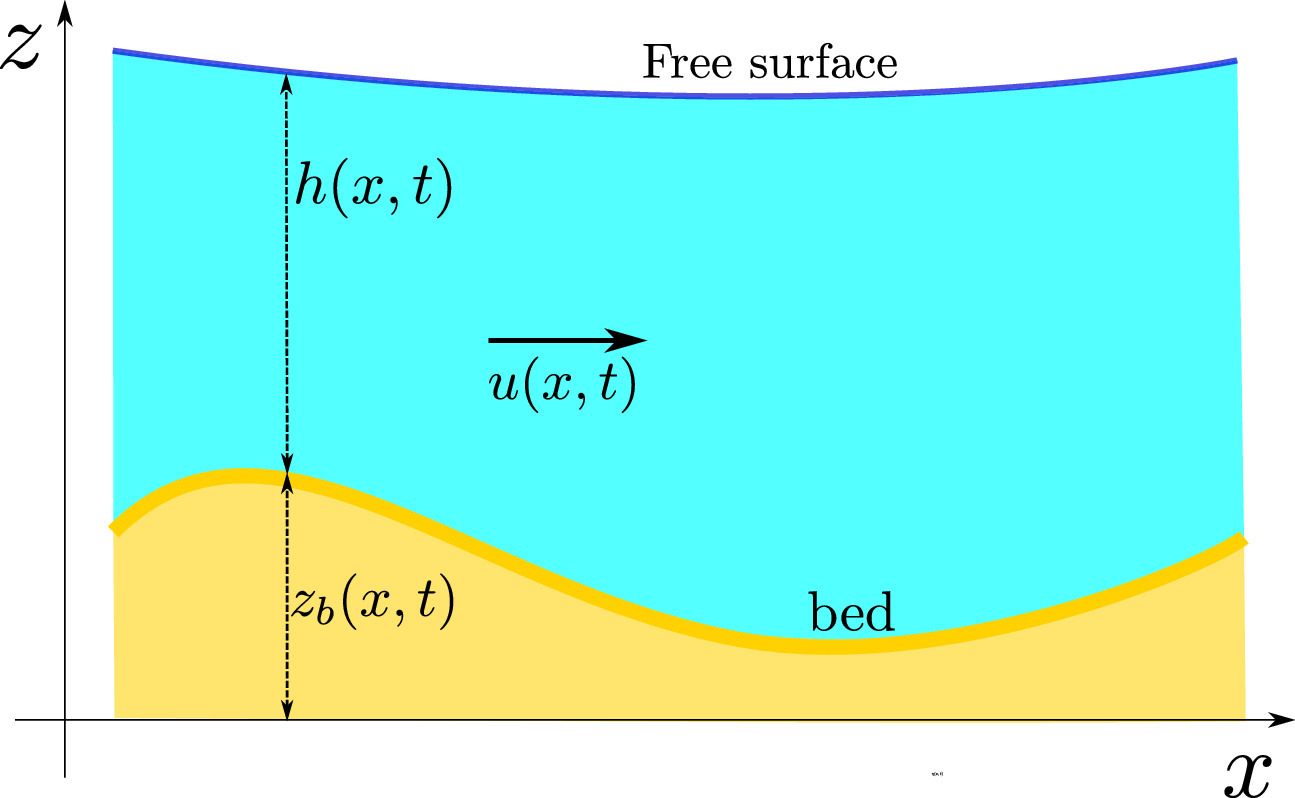
\includegraphics[width=10cm,height=6cm,keepaspectratio]{.//Pics//exner.jpg}
    \caption{Ecuación de Exner: evolución del lecho.}
    \end{figure}
\end{frame}

\begin{frame}{Ecuacion de Exner}
    \begin{align}
    {\partial z_b \over \partial t} + \frac{1}{1-\lambda_p} \nabla\cdot \mathbf{q_s} = E-D,
    \end{align}
    donde $q_s$ es el flujo sólido superficial $(m^2/s)$ y $E, D (m/s)$ son erosión y deposición. Para un modelo reducido, se puede usar:
    \begin{align}
        \mathbf{q_s}=\gamma_shC\mathbf{u}
    \end{align}
    y un cierre simple para erosión/deposición (prototipo):
    \begin{align}
        E-D=\beta_e\|\mathbf{u}\|-\beta_dC,
    \end{align}
    con $\beta_e,\beta_d$ ajustables. En escenarios iniciales, muchas veces se fija $E-D = 0$ para congelar el lecho y validar primero la dinámica; 
    luego se activa Exner.
\end{frame}

%/////////////////////////////////////////////%


%/////////////////////////////////////////////%
\section{Conclusiones} %Brian - Dylan
\begin{frame}{Conclusiones}
    \begin{enumerate}
        \item Un modelo de PDE acopladas da mucha mas fiabilidad a las predicciones, ya que sigue mejor la fisica
        \item Se pueden seguir agregando parametros y ecuaciones, aumentando la precision pero a la vez incrementando el costo computacional
    \end{enumerate}
\end{frame}



%/////////////////////////////////////////////%
\begin{frame}[allowframebreaks]{Referencias}
    \tiny
    \bibliographystyle{apacite}
    \bibliography{BibTesis}
\end{frame}

\end{document}